\chapter{A chapter with equations, chemical formula, figures and tables}
\label{chap_main}

The previous chapter \ref{chap_intro} contained only some text. Here some sample equations, chemical formula, figures, and tables
are introduced.

\section{Section with equations and chemical formula}
\label{sec_eq_fig_tab}

Materials science is highly interdisciplinary. So you will have to write complex equations some condensed-matter physicists use like:

\begin{equation}
\expval{\hat{O}}{\Psi_e} = \int \dotsc \int \Psi_e^{*}(x_1,\dotsc,x_N) \hat{O}
\Psi_e(x_1,\dotsc ,x_N)  dx_1 \dotsi dx_N
\quad .
\label{main_eq1}
\end{equation}

and,

\begin{equation}
\braket{\Psi_e} = \int \dotsc \int |\Psi_e (x_1,\dotsc,x_N)|^2  dx_1\dotsi dx_N = 1
\quad .
\label{main_eq2}
\end{equation}

Sometimes, you would also have to write chemical formula like chemists:

\begin{equation}
\centering
\ch{H3O_{aq}+ + 2 H2O <-> H5O2_{(aq)}+ + H2O <-> H7O3_{(aq)}+} \quad .
\label{main_eq3}
\end{equation}

With the appropriate tex packages defined, all this is possible.

\section{Section with tables and figures}
\label{sec_tab_figs}

Here are some sample tables and figures. For the table, I've taken data from my thesis and references \cite{Singh-miller2009, Sakong2018, Kittel1976, Salmeron1983}.

\begin{table}[!tbh]
\begin{center}
  \begin{tabular}{llc}
  \toprule
       &  a [\AA{}]  &  $\Phi\mathrm{_{Pt\hkl(111)}}$ [eV]  \\
  \midrule
  PBE (this work) &  3.97  &    5.69  \\
  PBE (ref. \cite{Singh-miller2009}) & 3.99  &    5.69   \\
  RPBE (this work) &  3.99 &   5.50 \\
  RPBE (ref. \cite{Sakong2018})&  3.99 &   5.51 \\
  Experiments &  3.92 \cite{Kittel1976} &   6.08 $\pm$ 0.15 \cite{Salmeron1983} \\
  \bottomrule
  \end{tabular}
\end{center}
\caption[Calculated lattice parameter of Pt and work function of the Pt\hkl(1 1 1) surface.]{The calculated lattice parameter of bulk Pt and the work function of the Pt\hkl(1 1 1) surface using different exchange-correlation functionals compared to experimental values.}
\label{main_tab1}
\end{table}

\begin{figure}[!tbh]
\centering
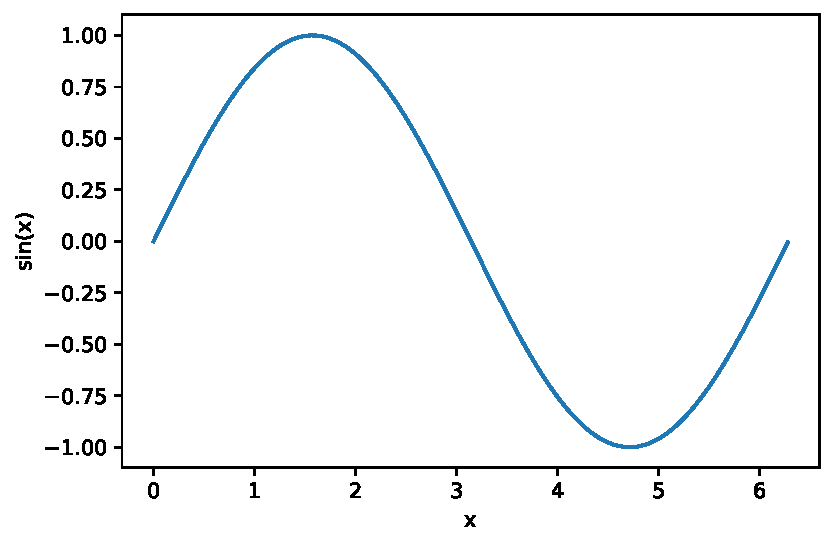
\includegraphics[scale=1., height=8cm]{\figpath/sinx.pdf}
\caption[A sinus curve]{A sinus curve to show how to include figures along with captions.} %The text in square brackets is what is rendered in the list of figures.
\label{main_fig1}
\end{figure}

Notice how in table \ref{main_tab1}, I've rendered crystallographic directions using the "miller" tex package.
